% ================================================================== PART I
\part{Physics: what we want and why it is hard}

\chapter{The project in one picture}

\section{The question}
Pressure is one of the most useful quantities in fluid mechanics. It sets the lift and drag on a body, drives cavitation, and is the source of flow noise. Yet it is surprisingly hard to measure over a whole field:
\begin{itemize}
  \item \textbf{Pressure taps} and transducers give pressure only at a few points, and only on walls.
  \item \textbf{Probes} placed in the flow disturb the very flow they measure.
  \item \textbf{Pressure-sensitive paint} works only on surfaces.
\end{itemize}
\textbf{Particle Image Velocimetry (PIV)}, by contrast, measures the \emph{velocity} over a whole plane without touching the flow. The question of this project is:

\begin{keyidea}[The question]
Given only PIV-type velocity fields $\uu(x,y,t)$ (noisy, smoothed, on a finite grid), how accurately can we reconstruct the pressure field $p(x,y,t)$, which algorithm should we use, and what controls the error?
\end{keyidea}

\section{The answer in three steps}
The momentum equation links pressure to velocity. Rearranged, it gives the pressure \emph{gradient} as a function of velocity only:
\begin{equation}
\nabla p = \G \equiv -\rho\frac{D\uu}{Dt} + \mu\nabla^2\uu .
\end{equation}
So the recipe is:
\begin{enumerate}
  \item \textbf{Differentiate} the measured velocity (in space and time) to get $\G$.
  \item \textbf{Integrate} $\G$ to get $p$ (up to an additive constant).
  \item \textbf{Compare} with a known true pressure to measure the error.
\end{enumerate}
Step 1 is where the difficulty lives: differentiation amplifies measurement noise. Step 2 decides whether that noise is averaged out or accumulated. Step 3 needs data where the true pressure is known, which is why the project uses exact Navier--Stokes solutions and a CFD simulation as ``virtual experiments''.

\begin{figure}[H]
\centering
\begin{tikzpicture}[node distance=5mm and 7mm, every node/.style={font=\small\sffamily},
  box/.style={draw=accent,fill=boxbg,rounded corners=2pt,align=center,minimum height=10mm,text width=27mm},
  hot/.style={draw=warn,fill=warnbg,rounded corners=2pt,align=center,minimum height=10mm,text width=27mm},
  ar/.style={-{Stealth[length=2.2mm]},thick,color=accent!80!black}]
\node[box] (src) {Velocity source\\ exact NS / CFD};
\node[box,right=of src] (piv) {Synthetic PIV\\ filter $W$, spacing $h$, noise $\sigma$};
\node[box,right=of piv] (den) {Optional\\ denoising};
\node[hot,below=9mm of den] (dudt) {Material derivative\\ $D\uu/Dt$ (Eul./Lagr.)};
\node[hot,left=of dudt] (G) {Pressure gradient\\ $\G=-\rho D\uu/Dt+\mu\nabla^2\uu$};
\node[box,left=of G] (int) {Integrate $\G$:\\ direct / omni / Poisson};
\node[box,below=9mm of int] (met) {Metrics vs exact $p$:\\ $\eps_{L2}$, maps, core};
\node[box,right=of met,text width=58mm] (sw) {Sweep one parameter at a time\\ ($h,\sigma,\Delta t$, BC, $W$, filter), 10 seeds each};
\draw[ar] (src)--(piv); \draw[ar] (piv)--(den); \draw[ar] (den)--(dudt); \draw[ar] (dudt)--(G); \draw[ar] (G)--(int); \draw[ar] (int)--(met); \draw[ar] (met)--(sw);
\end{tikzpicture}
\caption{The whole project as one pipeline. Orange boxes are where noise is amplified (differentiation); the integration step decides whether it is averaged out.}
\end{figure}

\section{What was built}
\begin{itemize}
  \item A Python package (about 7\,500 lines, NumPy/SciPy/Matplotlib) with three reconstruction algorithms: \textbf{direct integration}, \textbf{omni-directional integration} and a \textbf{pressure-Poisson solver}, plus five Poisson solvers (sparse direct, Jacobi, Gauss--Seidel, SOR, conjugate gradient).
  \item A \textbf{synthetic PIV model} that degrades exact velocity fields like a real PIV system: window averaging, finite spacing, random noise.
  \item \textbf{Validation flows}: the Taylor--Green vortex (stationary and convected) and Kovasznay flow (Re 20 and 40), all exact solutions of Navier--Stokes.
  \item A \textbf{CFD case}: a 2-D laminar cylinder wake at Re = 100 in OpenFOAM, on three meshes, sampled in a PIV-like window.
  \item \textbf{Studies} of grid spacing, noise, time step, boundary conditions, integration method, window size and denoising; a convergence and error-analysis study (norms, residuals, solver stability, scheme order).
  \item \textbf{87 unit tests}, all passing, which check every stencil, solver and parser against exact answers.
\end{itemize}

% ------------------------------------------------------------------
\chapter{Particle Image Velocimetry}

\section{How PIV works}
\begin{figure}[H]\centering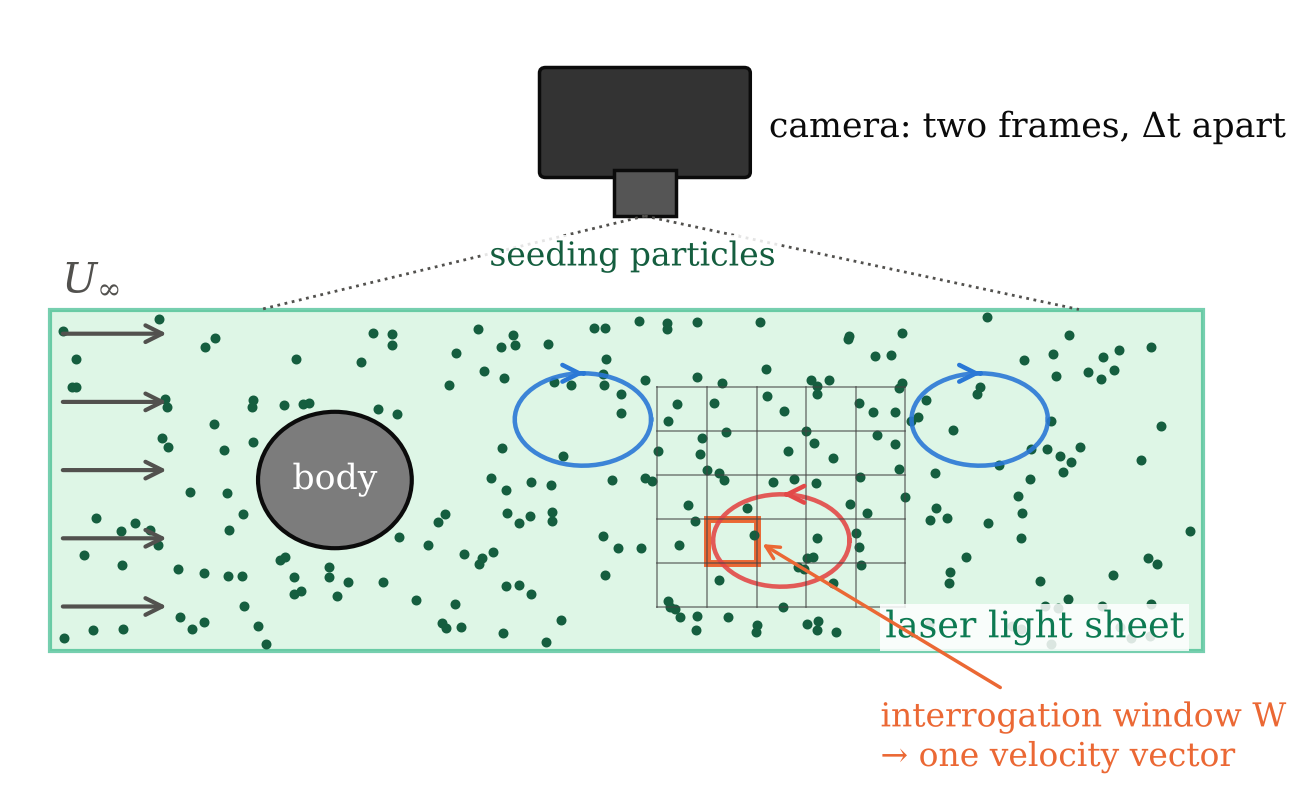
\includegraphics[width=0.62\linewidth]{img/f_piv_schematic.png}
\caption{Planar PIV. A laser sheet lights seeding particles; a camera records two frames $\Delta t$ apart; each interrogation window yields one velocity vector.}\end{figure}
\begin{enumerate}
  \item The flow is seeded with small tracer particles that follow it faithfully.
  \item A thin laser sheet illuminates a plane of the flow.
  \item A camera takes two images a short time $\Delta t$ apart.
  \item Each image is cut into small \textbf{interrogation windows} of size $W$. Cross-correlating a window in frame 1 with the same window in frame 2 gives the most likely particle displacement $\Delta\mathbf{x}$ in that window.
  \item The velocity of the window is $\uu = \Delta\mathbf{x}/\Delta t$. Repeating over all windows gives a vector field on a grid of spacing $h$ (often $h=W/2$ with 50\,\% overlap).
  \item \textbf{Time-resolved PIV} repeats this at high frame rate, giving a sequence of fields $\uu^{n-1},\uu^n,\uu^{n+1},\dots$ This is what the time derivative in $D\uu/Dt$ needs.
\end{enumerate}

\section{What PIV gets wrong}
Every pressure error in this project traces back to three properties of PIV data. The synthetic model in Chapter~8 reproduces exactly these three.
\begin{description}[style=nextline]
  \item[1. Spatial averaging (window $W$)] A vector is an average over the window, so it acts like a low-pass filter. Peaks are flattened and sharp gradients are smeared. For a box average of width $W$ the transfer function is $\sin(kW/2)/(kW/2)\approx 1-(kW)^2/24$, i.e.\ the measured velocity is biased by about $-(W^2/24)\nabla^2\uu$.
  \item[2. Finite spacing ($h$)] Derivatives must be estimated by finite differences on a grid of spacing $h$; their truncation error falls as $h^2$ but noise amplification grows as $1/h$ or $1/h^2$.
  \item[3. Random error ($\sigma$)] Correlation peaks are located with an uncertainty of order 0.1 pixel, giving a random velocity error typically 0.5--2\,\% of the flow speed. We model it as independent Gaussian noise of standard deviation $\sigma U$.
\end{description}
Real PIV adds further errors: out-of-plane motion (planar PIV misses $w$ and $\partial/\partial z$), particle lag, peak locking, and outliers. These are discussed as limitations in Chapter~14.

% ------------------------------------------------------------------
\chapter{From velocity to pressure: the governing equations}

\section{Pressure gradient from Navier--Stokes}
For an incompressible Newtonian fluid with constant density $\rho$ and viscosity $\mu$:
\begin{equation}
\nabla\cdot\uu = 0, \qquad
\rho\left(\frac{\partial\uu}{\partial t}+(\uu\cdot\nabla)\uu\right) = -\nabla p + \mu\nabla^2\uu .
\label{eq:ns}
\end{equation}
Solve the momentum equation for $\nabla p$:
\begin{equation}
\boxed{\;\nabla p = \G \equiv -\rho\frac{D\uu}{Dt}+\mu\nabla^2\uu, \qquad \frac{D\uu}{Dt}=\frac{\partial\uu}{\partial t}+(\uu\cdot\nabla)\uu\;}
\label{eq:G}
\end{equation}
In two dimensions, component by component (this is literally what \code{core/material\_derivative.py} computes):
\begin{align}
G_x &= -\rho\,(u_t + u\,u_x + v\,u_y) + \mu\,(u_{xx}+u_{yy}),\\
G_y &= -\rho\,(v_t + u\,v_x + v\,v_y) + \mu\,(v_{xx}+v_{yy}).
\end{align}
\begin{itemize}
  \item $D\uu/Dt$ is the \textbf{material (particle) acceleration}. It dominates at moderate and high Reynolds number.
  \item $\mu\nabla^2\uu$ is the \textbf{viscous term}. It matters at low Reynolds number: for Kovasznay flow at Re = 20 or 40, dropping it leaves an $O(1)$ error that never converges (a unit test checks this).
  \item In the non-dimensional CFD setup $\rho=1$, so $p$ is the \emph{kinematic} pressure $p/\rho$, exactly what OpenFOAM's incompressible solvers use.
\end{itemize}

\begin{keyidea}[Why this is an inverse problem]
Every term of $\G$ is a \emph{derivative} of measured data. So pressure from PIV is the inverse of differentiation: the data are differentiated (which amplifies noise) and then integrated (which can smooth it again). Everything else in the project is about doing these two operations well.
\end{keyidea}

\section{The material derivative: two ways to estimate it}

\subsection{Eulerian (fixed point)}
At a fixed grid node, with three snapshots $n-1,n,n+1$:
\begin{equation}
\left(\frac{D\uu}{Dt}\right)_E \approx \frac{\uu^{n+1}-\uu^{n-1}}{2\Delta t} + (\uu^n\cdot\nabla)\uu^n .
\end{equation}
The time difference has truncation error $-(\Delta t^2/6)\,\partial^3\uu/\partial t^3$: second order.

\subsection{Lagrangian (follow the particle)}
Instead of sitting at a point, follow a fluid particle along a straight path through the node with the local velocity $\mathbf{a}=\uu(\mathbf{x},t^n)$:
\begin{equation}
\left(\frac{D\uu}{Dt}\right)_L \approx \frac{\uu(\mathbf{x}+\mathbf{a}\Delta t,\,t^{n+1})-\uu(\mathbf{x}-\mathbf{a}\Delta t,\,t^{n-1})}{2\Delta t}.
\end{equation}
The velocities at the off-grid points come from cubic interpolation.

\textbf{Accuracy.} Let $L=\partial/\partial t+\mathbf{a}\cdot\nabla$ with $\mathbf{a}$ frozen. A shift in space and time is the exponential of $L$: $\uu(\mathbf{x}\pm\mathbf{a}\Delta t,t\pm\Delta t)=e^{\pm\Delta t L}\uu$. Then
\begin{equation}
\left(\frac{D\uu}{Dt}\right)_L=\frac{\sinh(\Delta t L)}{\Delta t}\uu = L\uu+\frac{\Delta t^2}{6}L^3\uu+O(\Delta t^4),
\end{equation}
and $L\uu$ is exactly $D\uu/Dt$. So the Lagrangian scheme is also second order in $\Delta t$; what differs is the \emph{size} of the error constant.

\begin{keyidea}[When Lagrangian wins]
Take a flow pattern $\mathbf{w}$ carried along at speed $\mathbf{c}$: $\uu(\mathbf{x},t)=\mathbf{c}+\mathbf{w}(\mathbf{x}-\mathbf{c}t)$.
\begin{itemize}
\item Eulerian error $\propto \partial^3\uu/\partial t^3 = -(\mathbf{c}\cdot\nabla)^3\mathbf{w}$, which scales like $c^3$.
\item Lagrangian error $\propto L^3\uu=(\mathbf{w}\cdot\nabla)^3\mathbf{w}$, which scales like $w^3$.
\end{itemize}
In a wake the vortices are \emph{carried} faster ($c\approx U$) than they \emph{spin} ($w<c$), so the Lagrangian estimate is more accurate at large $\Delta t$. For a stationary vortex ($c=0$) the Eulerian time error is almost zero and the Lagrangian one is larger. The project verifies both cases (Section~10.5).
\end{keyidea}

\begin{pitfall}[SciPy cubic interpolation]
Since SciPy 1.13, \code{RegularGridInterpolator(method="cubic")} computes spline coefficients with an iterative solver (atol $10^{-6}$). The interpolation error then stalls near $10^{-5}$ whatever the grid, and the Lagrangian error \emph{grows} under refinement. The code requests the direct solver (\code{solver=spsolve}), which restores fourth-order interpolation. Where the tracked point leaves the window, the code falls back to the Eulerian value and reports the fraction of such nodes.
\end{pitfall}

\section{The pressure-Poisson equation}
Taking the divergence of $\nabla p=\G$ gives an elliptic problem with Neumann boundary conditions:
\begin{equation}
\boxed{\;\nabla^2 p = \nabla\cdot\G \;\text{ in }\Omega, \qquad \frac{\partial p}{\partial n}=\n\cdot\G \;\text{ on }\partial\Omega\;}
\label{eq:poisson}
\end{equation}

\subsection{Compatibility}
Integrate the Poisson equation over the domain and use Gauss's theorem: $\iint_\Omega\nabla^2p\,dA=\oint_{\partial\Omega}\partial p/\partial n\,ds$. A solution exists only if
\begin{equation}
R \equiv \iint_\Omega\nabla\cdot\G\,dA-\oint_{\partial\Omega}\n\cdot\G\,ds = 0 .
\end{equation}
For an exact gradient field $R=0$ automatically. For discretised or noisy $\G$ it is not, and the code reports $R$ (\code{compatibility\_residual}). Even when it holds, the solution is unique only up to a constant: adding any constant to $p$ changes nothing.

\subsection{Poisson as a least-squares projection}
Measured $\G$ is not exactly a gradient: it has a non-zero curl, which can only be error (the curl of a true gradient is zero). What is the ``best'' pressure? Minimise the mismatch
\begin{equation}
J[p]=\iint_\Omega|\nabla p-\G|^2\,dA .
\end{equation}
The calculus of variations gives the Euler--Lagrange equation $\nabla^2p=\nabla\cdot\G$ in $\Omega$ and the natural boundary condition $\partial p/\partial n=\n\cdot\G$ on $\partial\Omega$: exactly Eq.~\eqref{eq:poisson}.

\begin{keyidea}[Why Poisson is robust]
The Poisson problem \emph{projects} the measured $\G$ onto the space of gradient fields. It keeps the curl-free part and discards the curl, which is pure error. That is why Poisson reconstruction is path-independent and filters noise, and why the source term and the boundary data must come from the \emph{same} $\G$ (Section~10.3 shows what happens otherwise).
\end{keyidea}

\subsection{An alternative source term (2-D incompressible identity)}
Take the divergence of $\G$ term by term. $\nabla\cdot(\partial\uu/\partial t)=\partial(\nabla\cdot\uu)/\partial t=0$ and $\nabla\cdot\nabla^2\uu=\nabla^2(\nabla\cdot\uu)=0$. Only the convective term survives:
\begin{equation}
\nabla\cdot((\uu\cdot\nabla)\uu)=(\partial_iu_j)(\partial_ju_i)+u_j\partial_j(\partial_iu_i)=u_x^2+2u_yv_x+v_y^2,
\end{equation}
so
\begin{equation}
\nabla^2p=-\rho\left(u_x^2+2u_yv_x+v_y^2\right).
\end{equation}
This form needs no time derivative and no viscous term, which looks attractive. But it assumes $\nabla\cdot\uu=0$ exactly (noisy PIV data are not solenoidal), it multiplies noisy derivatives together (a bias of order $\sigma^2/h^2$), and its boundary data still come from $\G$. Section~10.3 shows that it is 5--8$\times$ worse on noisy data.

\textit{Check on Taylor--Green:} $u_x=-\sin x\sin y\,F$, $v_y=\sin x\sin y\,F$, $u_y=\cos x\cos y\,F$, $v_x=-\cos x\cos y\,F$, so $-\rho(2\sin^2x\sin^2y-2\cos^2x\cos^2y)F^2=\rho(\cos2x+\cos2y)F^2=\nabla^2p$. \checkmark

\section{Bernoulli boundary values}
For \textbf{steady, irrotational} flow, $p+\tfrac12\rho|\uu|^2$ is constant along the whole field, so a free-stream edge could be given the Dirichlet value
\begin{equation}
p=p_\infty+\tfrac12\rho\,(U_\infty^2-|\uu|^2).
\end{equation}
For unsteady irrotational flow the correct form is $p+\rho\,\partial\phi/\partial t+\tfrac12\rho|\uu|^2=\text{const}$, and in rotational flow there is no such relation at all. Both validation flows carry vorticity everywhere, so Bernoulli edges \emph{must} fail there; the project tests this deliberately (Section~10.4).

\begin{viva}
\begin{enumerate}[leftmargin=*]
\item \emph{Why can't PIV measure pressure directly?} It measures particle displacement, i.e.\ velocity. Pressure enters only through the momentum equation.
\item \emph{Why is the result only defined up to a constant?} Only $\nabla p$ is known; a constant has zero gradient. We compare $p-\bar p$ with $p_{ref}-\bar p_{ref}$.
\item \emph{When can you neglect the viscous term?} At high Reynolds number away from walls; never in Kovasznay flow at Re 20--40.
\item \emph{What does the compatibility condition mean physically?} The total ``source'' inside must equal the net flux through the boundary; a non-gradient $\G$ violates it.
\item \emph{Why does Poisson filter noise?} It is the least-squares fit of a gradient field to $\G$; the curl part (pure error) is discarded.
\end{enumerate}
\end{viva}
